\chapter{Xây dựng hệ thống IoT và thiết kế ngôn ngữ truy vấn ngữ nghĩa}

\section{Xây dựng hệ thống IoT}
\subsection{Phần cứng}

Các thiết bị IoT được cài đặt trên 3 khu vực trong phòng 609 thư viện Tạ Quang Bửu. Trong mỗi phòng, có một máy tính nhỏ Raspberry Pi 3, cài đặt nền tảng IoT để quản lý các thiết bị trong phòng. Trong mỗi phòng, gồm :
\begin{itemize}
	\item Một cảm biến chuyển động
	\item Một cảm biến ánh sáng
	\item Một cảm biến nhiệt độ, độ ẩm
	\item Ba đèn LED tượng trưng cho ba thiết bị IoT có khả năng thiết lập các trạng thái khác nhau (bật/tắt).
\end{itemize}
Các thiết bị trong mỗi phòng được gom thành hai "vật" tương ứng với hai hộp. "Vật" 1 chứa cảm biến chuyển động và ba đèn LED; "vật" 2 chứa cảm biến ánh sáng, cảm biến nhiệt độ-độ ẩm. 
\clearpage

\begin{figure}
	\center
	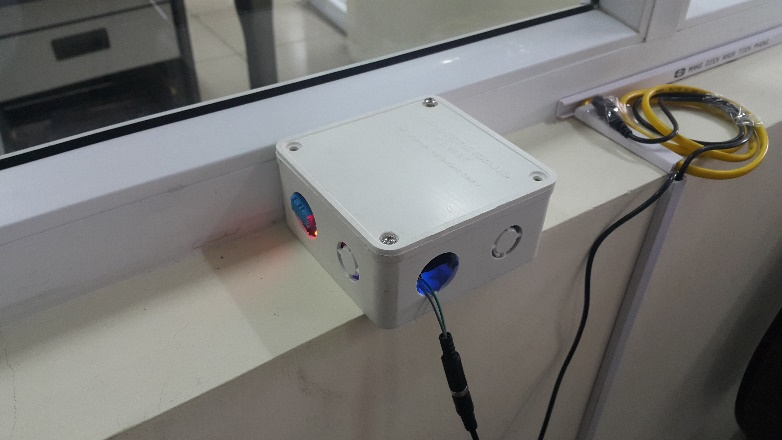
\includegraphics[scale=1]{image/hop_1}
	\label{fig:2hop}
	%\caption{Hai hộp đại diện cho hai "vật"}
\end{figure}

\begin{figure}
	\center
	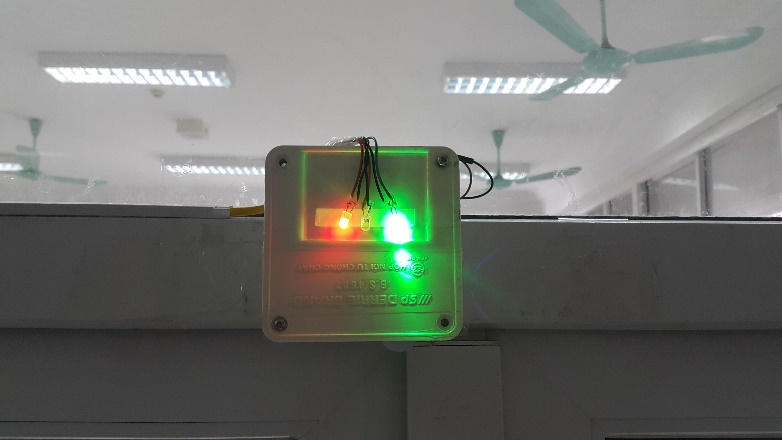
\includegraphics[scale=1]{image/hop_2}
	\label{fig:2hop}
	\caption{Hai hộp đại diện cho hai "vật"}
\end{figure}

Để lấy được dữ liệu từ các thiết bị trên, ta sử dụng board vi mạch xử lý Arduino Uno. Tuy nhiên, vi mạch này không có chức năng gửi dữ liệu thông qua mạng wifi, do đó, cần phải lắp thêm module ESP8266 để gửi dữ liệu từ Arduino, qua ESP8266 rồi gửi lên platform.

\subsection{Các giao thức sử dụng}
Giao thức được dùng để truyền tải dữ liệu từ ESP8266 lên nền tảng IoT là MQTT thông qua mạng wifi. MQTT (Message Queuing Telemetry Transport) là một giao thức gửi dạng publish/subscribe sử dụng cho các thiết bị IoT với băng thông thấp, độ tin cậy cao và khả năng được sử dụng trong mạng lưới không ổn định. Trong đó, broker được coi như trung tâm, nó là điểm giao của tất cả các kết nối đến từ client. Nhiệm vụ chính của broker là nhận message (gói tin) từ publisher, xếp các message theo hàng đợi rồi chuyển chúng tới một địa chỉ cụ thể. Nhiệm vụ phụ của broker là nó có thể đảm nhận thêm một vài tính năng liên quan tới quá trình truyền thông như: bảo mật message, lưu trữ message, logs,...
Client thì được chia thành 2 nhóm là publisher và subscriber. Client là các chương trình được thiết kế để có thể hoạt động một cách linh hoạt (lightweight). Client chỉ làm ít nhất một trong 2 việc là publish các message lên một topic cụ thể hoặc subscribe một topic nào đó để nhận message từ topic này.

Các khái niệm đáng chú ý trong giao thức MQTT
Message
Trong giao thức MQTT, message còn được gọi là "message payload", có định dạng mặc định là plain-text (chữ viết người đọc được), tuy nhiên người sử dụng có thể cấu hình thành các định dạng khác.
Topic
Topic có thể coi như một "đường truyền" logic giữa 2 điểm là publisher và subscriber. Về cơ bản, khi message được publish vào một topic thì tất cả những subscriber của topic đó sẽ nhận được message này.
%\clearpage
\begin{figure}[h]
	\center
	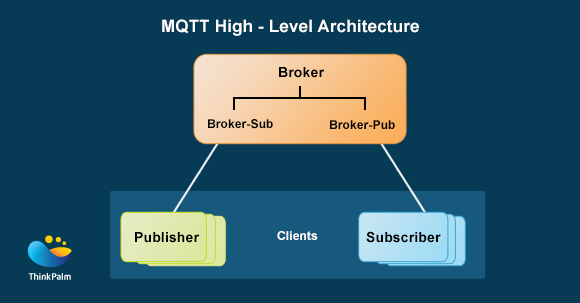
\includegraphics[scale=0.6]{image/mqtt}\\
	\caption{Giao thức truyền tin MQTT}
	Nguồn: https://techmaster.vn/posts/34394/iot-giao-thuc-mqtt-va-ung-dung-trong-iot
\end{figure}
Mô hình triển khai:
\clearpage
\begin{figure}[h!]
	\center
	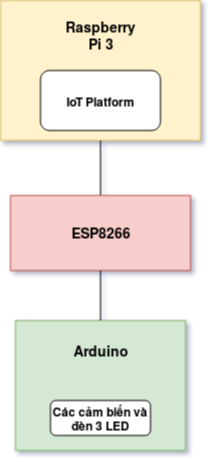
\includegraphics[scale=0.6]{image/mo_hinh_trien_khai_phan_cung}
	\caption{Mô hình triển khai phần cứng}
	
	\label{fig:mo_hinh_trien_khai_phan_cung}
\end{figure}

Hệ thống triển khai thực tế :\\

\begin{figure}[h!]
	\center
	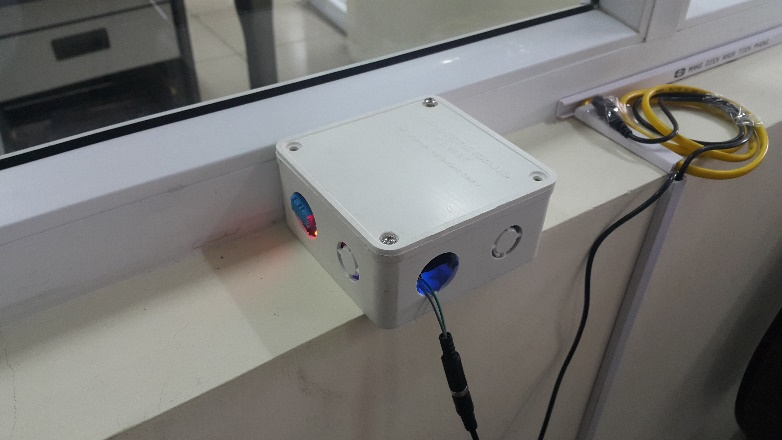
\includegraphics[scale=1]{image/hop_1}
	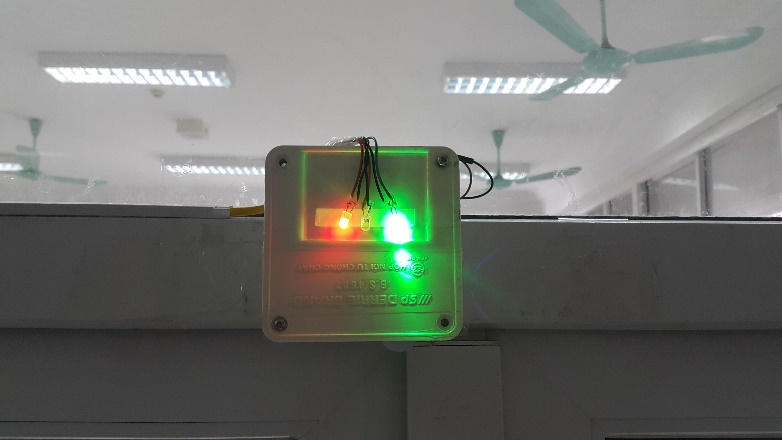
\includegraphics[scale=1]{image/hop_2}
\end{figure}

\begin{figure}[h!]
	\center
	%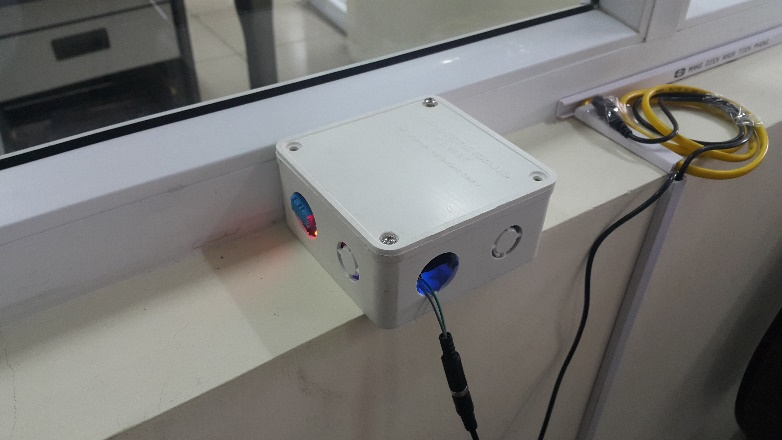
\includegraphics[scale=1]{image/hop_1}
	%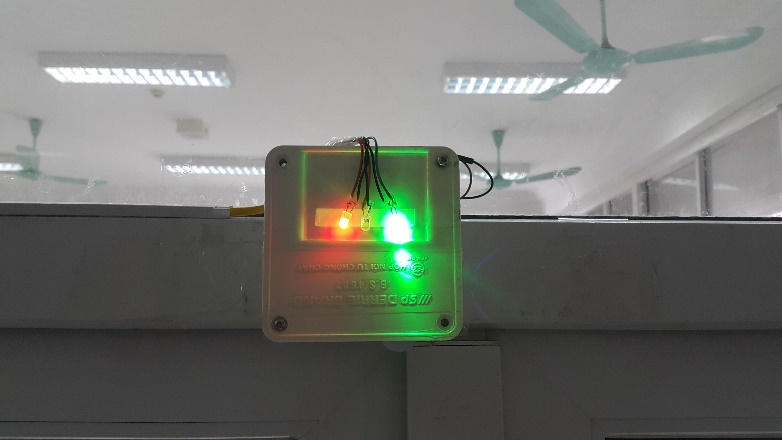
\includegraphics[scale=1]{image/hop_2}
	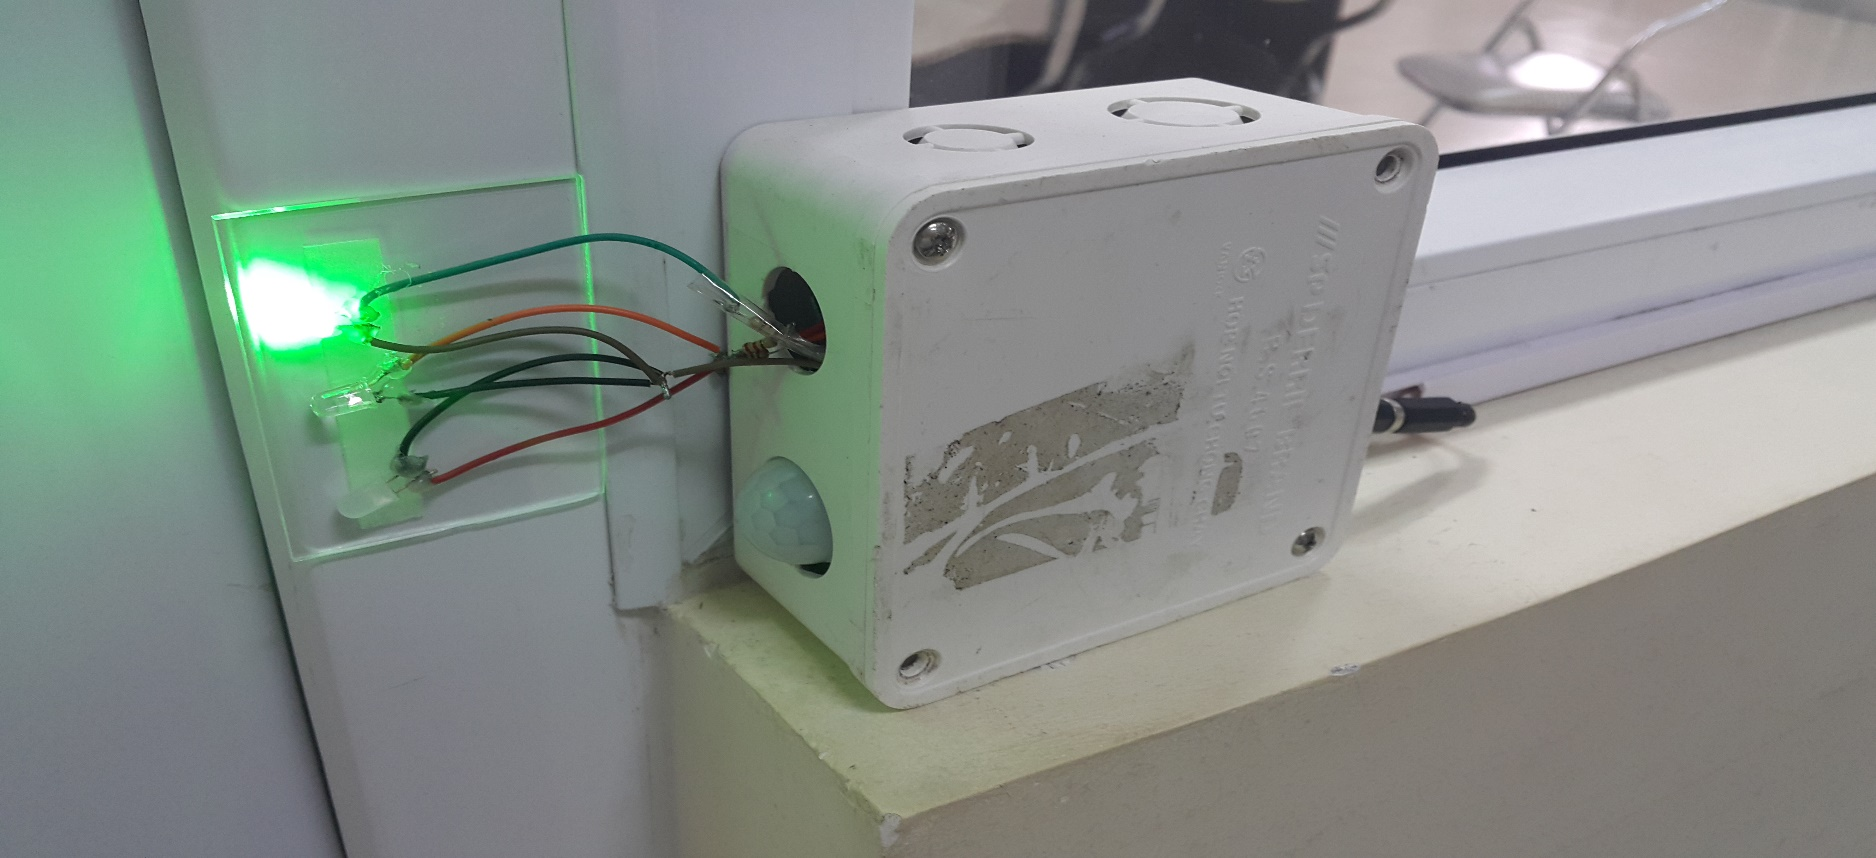
\includegraphics[scale=0.4]{image/hop_3}	
	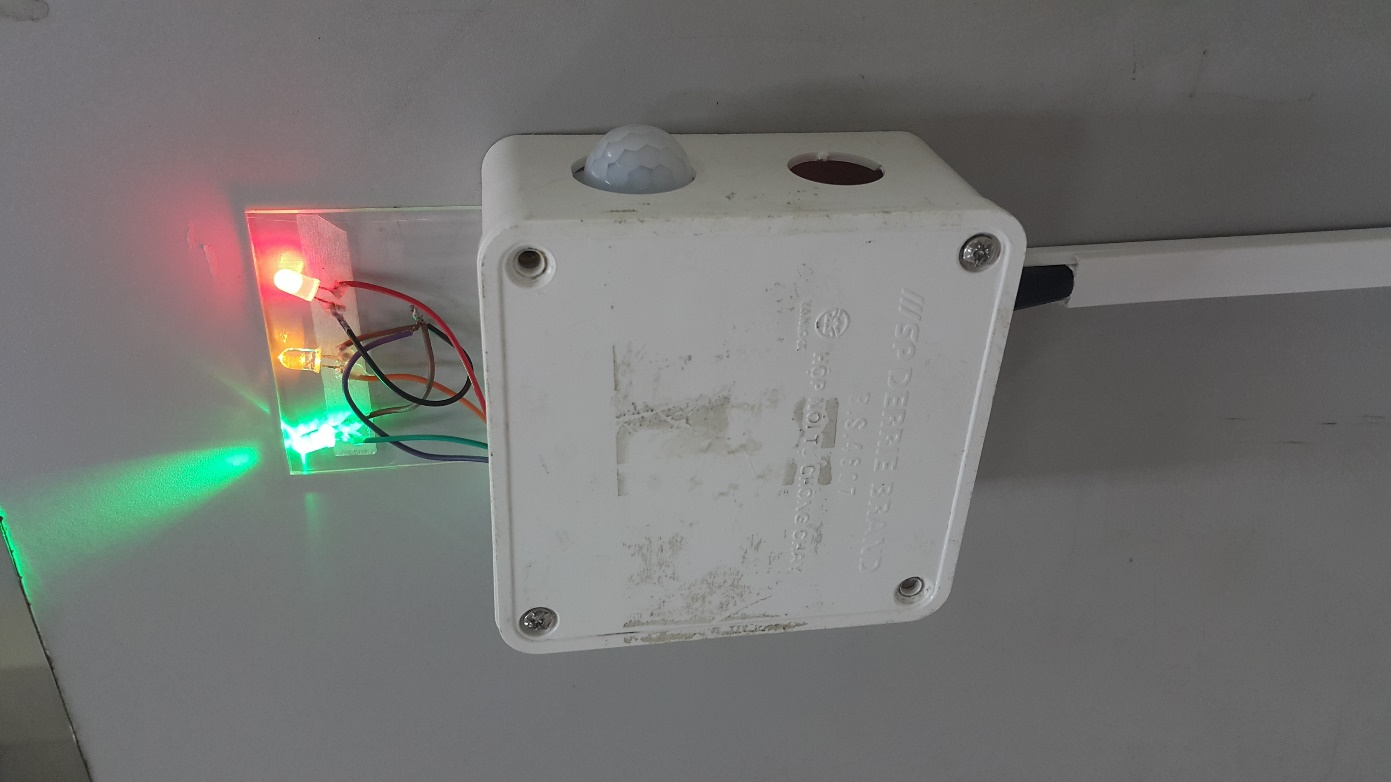
\includegraphics[scale=0.5]{image/hop_4}
	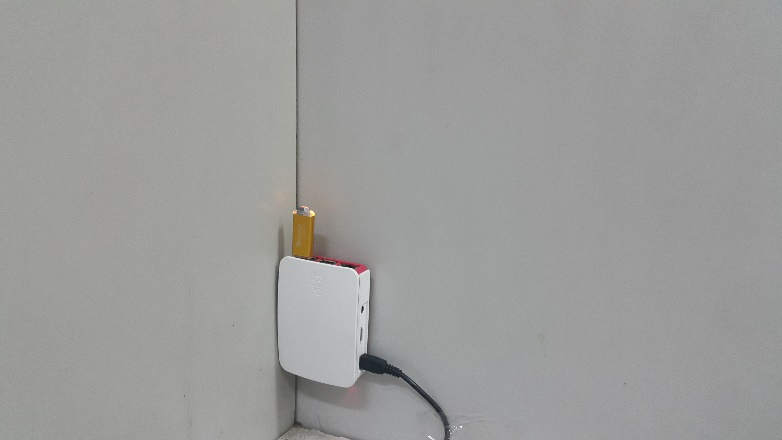
\includegraphics[scale=1]{image/hop_5}
	\caption{Triển khai phần cứng trên phòng 609 Thư viện TQB}
	\label{fig:trien_khai_phan_cung}
\end{figure}
%\clearpage 


\subsection{Các nền tảng IoT sử dụng}
Hiện nay, trong thực tế có rất nhiều các nền tảng IoT được sử dụng, cả các platform nguồn đóng và nguồn mở. Các nền tảng IoT mã nguồn đóng thường được các công ty hoạt động vì lợi nhuận xây dựng, ví dụ như IBM, Amazon, ... còn các nền tảng IoT mã nguồn mở thường được cộng đồng mã nguồn mở hoặc các công ty hoạt động phi lợi nhuận xây dựng. Do đề tài chỉ mang mục đích nghiên cứu, nên tôi sử ba nền tảng IoT mã nguồn mở để mô tả tính không đồng nhất về cấu trúc dữ liệu của các platform và cách ánh xạ các cấu trúc không đồng nhất này về dạng chuẩn chung của ontology. Ba platform được sử dụng là OpenHAB, HomeAssistant và ThingsBoard.

OpenHAB là một nền tảng IoT được dùng chủ yếu để quản lý các thiết bị trong ngôi nhà thông minh. Các ưu điểm của OpenHAB là:
\begin{itemize}
	\item Có khả năng tích hợp các thiết bị, hệ thống khác.
	\item Cung cấp giao diện thống nhất cho người dùng và người dùng có thể tạo ra các luật dựa trên thông tin của các thiết bị trong hệ thống.
	\item Cung cấp một công cụ linh động để tạo ra một ngôi nhà tự động. OpenHAB hỗ trợ tự thêm rất nhiều loại thiết bị, giao thức phổ biến trong IoT. 
\end{itemize}
OpenHAB cung cấp tập các Restful API để các chương trình khác có thể sử dụng để lấy thông tin về các thiết bị hoặc ra lệnh cho các thiết bị.
%\clearpage

\begin{figure}[h!]
	\center
	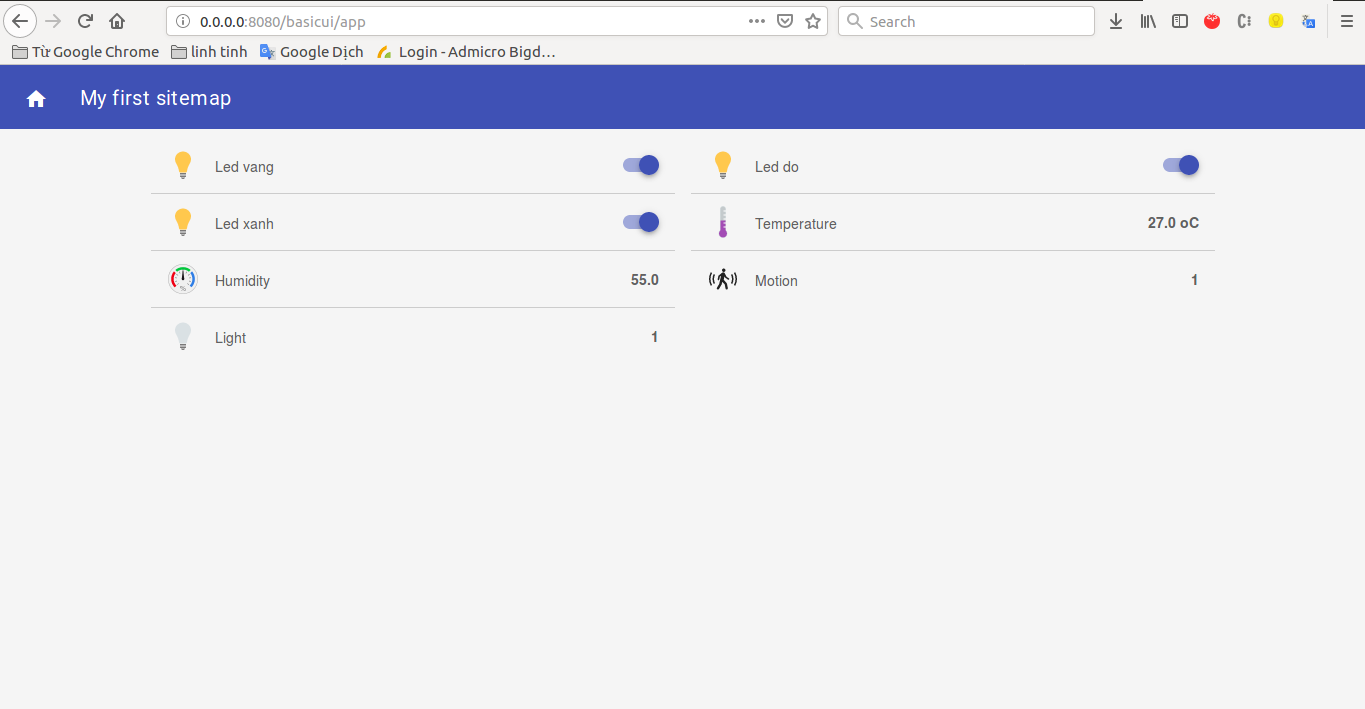
\includegraphics[scale=0.3]{image/openhab} \\
	\caption{Giao diện quản lý thiết bị của platform OpenHAB}
	\label{fig:giao_dien_openhab}
\end{figure}

Home Assistant là một nền tảng IoT mã nguồn mở ưu tiên quản lý các thiết bị trong ngôi nhà thông minh và có quan tâm tới tính riêng tư. Được cộng đồng lớn mạnh trên thế giới phát triển. Home Assistant phù hợp chạy trên Raspberry Pi hoặc một máy chủ tại chỗ. Home Assistant cũng lượng lớn hỗ trợ các thiết bị thông minh trên thị trường cũng như các giao thức phổ biến được sử dụng trong IoT. Giống với OpenHAB, Home Assistant cũng cung cấp các Restful API để lấy dữ liệu của thiết bị, đồng thời điều khiển các thiết bị qua các API này.
\clearpage

\begin{figure}[h!]
	\center
	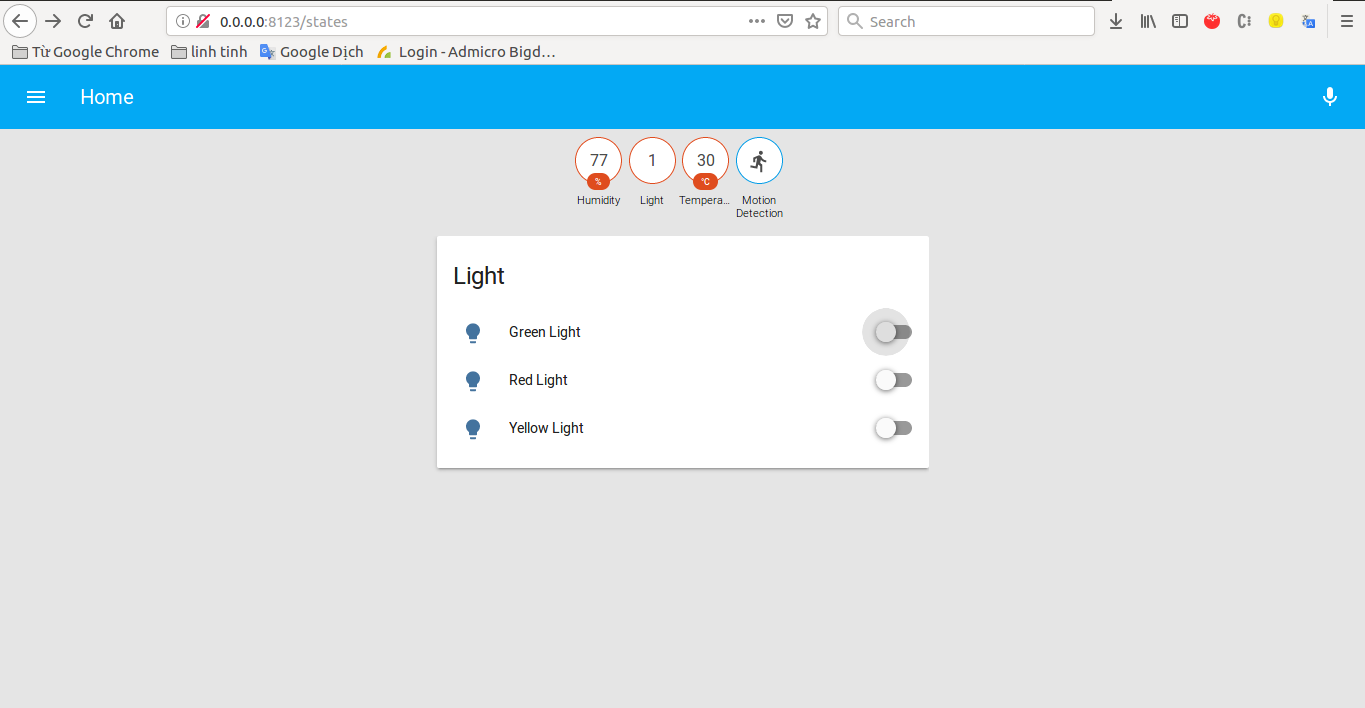
\includegraphics[scale=0.3]{image/homeassistant} \\
	\caption{Giao diện quản lý thiết bị của platform Home Assistant}
	\label{fig:giao_dien_homeassistant}
\end{figure}


Thingsboard là một nền tảng IoT mã nguồn mở giúp thu thập dữ liệu, xử lý,trực quan hóa dữ liệu và quản lý các thiết bị. Nó cho phép kết nối các thiết bị thông qua các giao thức chuẩn của IoT như MQTT, CoAp, HTTP. Thingsboard đảm bảo tính mở rộng, tính chịu lỗi và hiệu năng nên người dùng không sợ bị mất dữ liệu. Không giống như OpenHAB chưa có tính bảo mật dữ liệu, hay cơ chế bảo mật yếu Home Assistant, Thingsboard có cơ chế bảo mật dữ liệu của các thiết bị thông qua Token. Để truy cập được vào các thiết bị, bắt buộc phải biết token của các thiết bị này.

\begin{figure}[h!]
	\center
	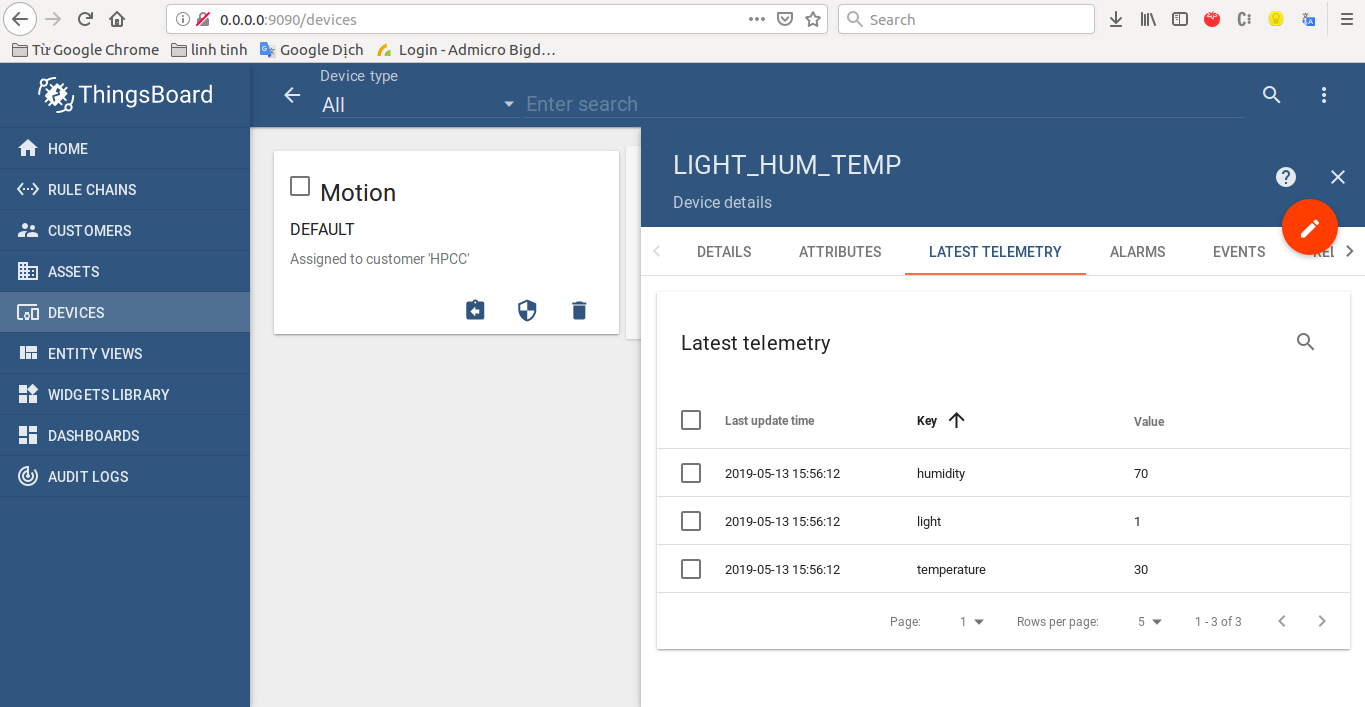
\includegraphics[scale=0.3]{image/thingsboard} \\
	\caption{Giao diện quản lý thiết bị của platform Thingsboard}
	\label{fig:giao_dien_thingsboard}
\end{figure}


\section{Thiết kế ngôn ngữ truy vấn cho IoT}

\subsection{Xây dựng ontology}
Tuân theo các nguyên tắc và các bước xây dựng ontology, tôi thực hiện việc xây dựng ontology theo các bước sau:

\underline{Bước 1:} Xác định lĩnh vực và phạm vi của ontology \\
Lĩnh vực cần xây dựng ontology là IoT. Tuy nhiên, lĩnh vực IoT rất rộng lớn, gồm đa dạng các thiết bị, cảm biến và gồm nhiều khái niệm. Do đó, việc giới hạn phạm vi xây dựng ontology trong đề tài này là công việc quan trọng. Từ đó, tôi giới hạn phạm vi nghiên cứu của đề tài là lĩnh vực IoT trong nhà thông minh gồm có các thành phần: các cảm biến, các thiết bị, các nền tảng IoT, các ứng dụng/phạm vi sử dụng các nền tảng IoT. 
Mục đích sử dụng của ontology là để tạo ra các câu truy vấn ngữ nghĩa đơn giản. Một số câu hỏi ontology cần có thể trả lời được như:
\begin{itemize}
	\item Một khái niệm có những thuộc tính tương ứng nào?
	\item Một thực thể có các mối quan hệ với các thực thể nào khác?
	\item ...
\end{itemize}
Ngoài ra, ontology cũng cần có khả năng mở rộng so với các thành phần trong ngôi nhà thông minh. 

\underline{Bước 2:} Xem xét việc kế thừa các Ontology có sẵn: \\
Trong các ontology về IoT, SSN ontology là ontology được nhắc đến rất phổ biến. Ontology này mô tả các cảm biến, các quan sát và các khái niệm liên quan. Nó không mô tả các thành phần như thời gian, địa điểm, ... Những thành phần này, có thể được thêm vào từ các ontology khác thông qua ngôn ngữ OWL (Web Ontology Language).
SSN ontology được phát triển bởi W3C Semantic Sensor Network Incubator Group (SSN-XG). Việc thiếu các khái niệm để mô tả cụ thể các loại cảm biến, đơn vị của các giá trị thu được, thời gian, địa điểm, ... khiến cho SSN ontology khó tích hợp được vào các lĩnh vực cụ thể mà đôi khi không theo chuẩn chung.
%\clearpage

\begin{figure}[h!]
	\center
	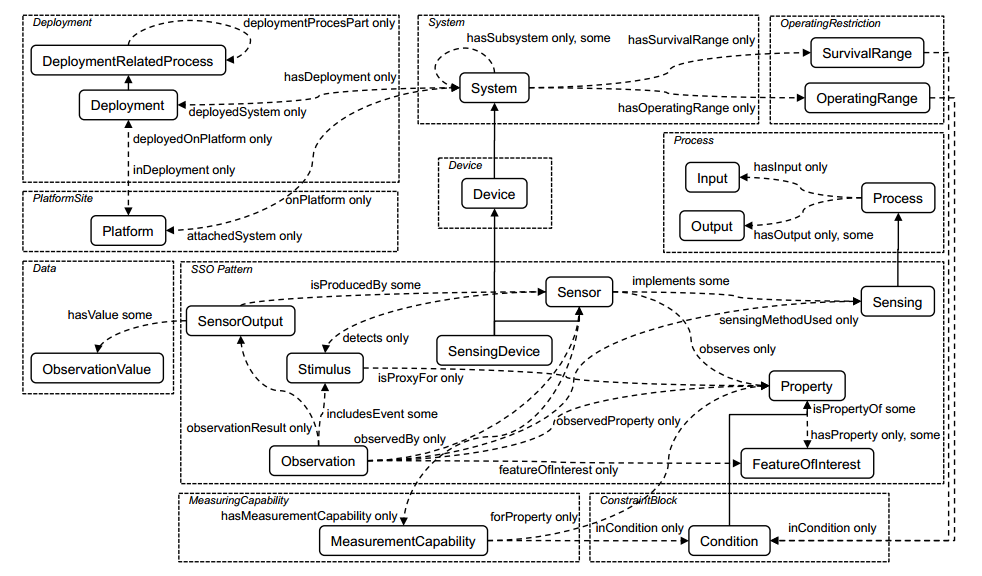
\includegraphics[scale=0.4]{image/ssn_ontology} \\
	\caption{SSN ontology}
	\small nguồn: https://corescholar.libraries.wright.edu/knoesis/610/?utm\_source=corescholar.libraries.wright.edu \%2Fknoesis\%2F610\&utm\_medium=PDF\&utm\_campaign=PDFCoverPages
\end{figure}

Một ontology khác là ontology IoT-A, cung cấp các khái niệm chính như Service, và các khái niệm chủ yếu theo liên quan tới các Service. Nó chỉ tái sử dụng khái niệm ssn:condition. Hơn nữa, nó rất phức tạp, không sử dụng các ontology chuẩn, và gặp nhiều vấn đề về tính dư thừa. 
\clearpage

\begin{figure}[h!]
	\center
	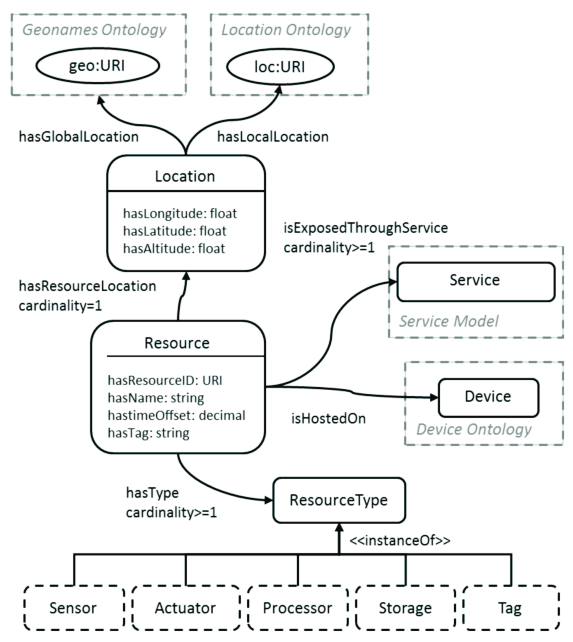
\includegraphics[scale=0.5]{image/iot-a}
	\caption{IoT-A ontology}
	nguồn: https://www.researchgate.net/profile/Suparna\_De/publication/330729011/figure/fig1/ AS:720756187090946@1548853074205/Internet-of-Things-Architecture-IoT-A-Resource-Model.png
\end{figure}

IoT-Lite ontology là một ontology rút gọn của SSN ontology để biểu diễn các tài nguyên, thực thể và các dịch vụ trong IoT. Sự rút này cho phép IoT-Lite không quá lớn và không cần thời gian dài để xử lý khi thực hiện một truy vấn trên ontology này. Tuy nhiên, nó cũng cho phép khả năng mở rộng để biểu diễn các khái niệm trong IoT một cách chi tiết hơn, trong các lĩnh vực khác. Nó cũng có thể được kết hợp với các ontology biểu diễn dữ liệu IoT dạng stream như SAO ontology. 
\clearpage

\begin{figure}[h!]
	\center
	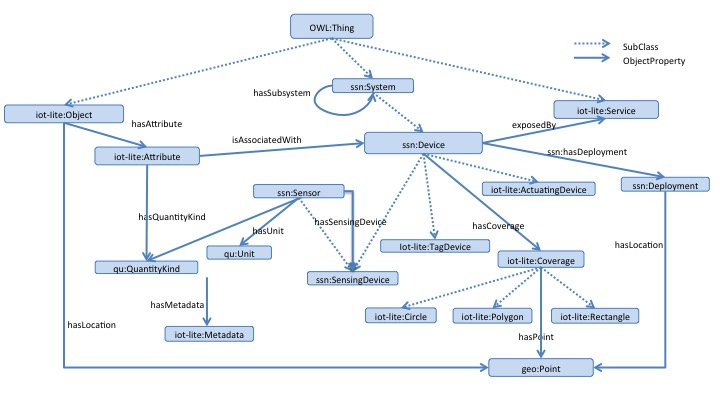
\includegraphics[scale=0.6]{image/iot-lite} \\
	\caption{IoT-Lite ontology}
	nguồn: https://www.w3.org/Submission/2015/SUBM-iot-lite-20151126/figures/Ontology.jpg
\end{figure}


Mặc dù đã tồn tại nhiều ontology, tuy nhiên, các ontology này chủ yếu được viết theo ngôn ngữ RDF, OWL dựa trên nền tảng web. Hơn nữa, các ontology này khá phức tạp, không phù hợp với phạm vi của đề tài. Do đó, tôi chỉ kế thừa các khái niệm, thuộc tính và các mối quan hệ trong các ontology này để xây dựng ontology của mình.

\underline{Bước 3:} Liệt kê các thuật ngữ quan trọng trong Ontology	\\
Một số khái niệm quan trọng trong lĩnh vực nhà thông minh: 
\begin{itemize}
	\item Smart Context: là một phạm vi triển khai hoặc một ứng dụng trong IoT. Đây sẽ là thành phần trên nhất trong cây phân cấp các khái niệm. Một smart context có thể chứa các smart context khác; một smart context cũng có thể nằm trong một smart context khác.
	\item Platform: là một phần mềm gồm nhiều thành phần, cho phép kết nối, quản lý và tự động hóa việc kết nối các thiết bị trong môi trường IoT. Nó kết nối các thiết bị phần cứng với nhau, cũng như với cloud bằng việc sử dụng linh hoạt các giao thức kết nối, cung cấp các cơ chế bảo mật và cung cấp năng lực xử lý dữ liệu.
	\item Source: Là một thiết bị vật lý hoặc thiết bị ảo. Source sẽ sinh ra dữ liệu về môi trường hay bất kỳ thứ gì mà nó theo dõi. Một Source có thể là một Thing, Gateway hay một Process Unit.
	\item Thing: Là một thiết bị, bao gồm một hoặc một tập hợp các cảm biến
	\item Gateway: Là một thiết bị vật lý hay một trình phần mềm phục vụ như là một điểm kết nối giữa các thiết bị thông minh, các cảm biến với cloud.
	\item Container: Là một thiết bị ảo để theo dõi các tài nguyên trong một hệ thống IoT như CPU, RAM, ổ đĩa, …
	\item Log: là dữ liệu được sinh ra từ Source. Các tệp tin log có thể được dùng để lấy ra các thông tin lịch sử của dữ liệu, trạng thái theo dõi các thiết bị, …
	\item Metric được sử dụng để nhấn mạnh các loại độ đo khác nhau của dữ liệu trong IoT.  Một số loại Metric có thể như Enumeration, Gauge, Counter, Histogram, Summary. Mỗi Metric có các đơn vị tương ứng như Percent, Time, Degree. Mỗi Source đều có một hoặc nhiều Metric của nó.
	\item Data Point: Được tạo ra khi một Source hoạt động. Dựa trên thông tin về Metric của một Source, dữ liệu sẽ có DataType, DataValue phù hợp.
\end{itemize}
\underline{Bước 4:} Xây dựng các lớp/khái niệm và cấu trúc lớp/khái niệm phân cấp: \\
Xây dựng theo kiểu trên xuống, ta nhận thấy Smart Context là khái niệm có mức độ tổng quát cao nhất, là gốc của đồ thị. Các khái niệm Log, Platform, Source, Metric, Data Point là các khái niệm trung gian. Các khái niệm Thing, Gateway, Container, Percent, Time, Degree, … là các khái niệm lá. 

\underline{Bước 5:} Định nghĩa các thuộc tính và quan hệ cho lớp:	\\
Các thuộc tính của các khái niệm trong ontology:
\hspace{0mm}Smart context có các thuộc tính:
\begin{itemize}
	\item SmartContextId: định danh duy nhất của một smart context
	\item SmartContextName: tên của một smartcontext
\end{itemize} 

\hspace{0mm}Platform có các thuộc tính:
\begin{itemize}
	\item PlatformId: định danh duy nhất của một platform
	\item PlatformName: tên của platform
	\item PlatformType: loại platform
	\item PlatformHost: địa chỉ của máy cài đặt platform này
	\item PlatformPort: Cổng cài đặt platform	
	\item PlatformStatus: trạng thái hoạt động của platform
\end{itemize}

\hspace{0mm}Source có các thuộc tính:
\begin{itemize}
	\item SourceId: Định danh toàn cục duy nhất của một Source
	\item EndPoint: Địa chỉ của Source
	\item SourceStatus: Trạng thái hoạt động của Source
	\item Description: Mô tả về Source
	\item SourceType: loại Source	
	\item Label: nhãn của Source
	\item LocalId: Địa chỉ cục bộ của Source
\end{itemize}



\hspace{0mm}Metric có các thuộc tính:
\begin{itemize}
	\item MetricId: định danh toàn cục duy nhất của một Metric
	\item MetricName: tên của một Metric
	\item MetricLocalId: định danh cục bộ của một Metric
	\item MetricType: loại Metric
	\item Unit: đơn vị của Metric
	\item ValueDomain: trường giá trị để ánh xạ các khác nhau trong việc biểu diễn các giá trị dữ liệu của cùng một thiết bị nhưng trong các platform khác nhau. Ví dụ, cùng một cảm biến nhiệt độ, nhưng OpenHAB biểu diễn giá trị của nó là 0/1, HomeAssistant biểu diễn giá trị là on/off.
\end{itemize}


\hspace{0mm}Data Point có các thuộc tính:
\begin{itemize}
	\item DataPointId: định danh duy nhất của một Data Point
	\item DataType: Kiểu dữ liệu của một Data Point
	\item time: thời điểm Data Point được thu nhận
	\item value: giá trị của Data Point
\end{itemize}


\hspace{0mm}Log có các thuộc tính:
\begin{itemize}
	\item time: thời điểm ghi log
	\item message: nội dung của log
\end{itemize}

\hspace{0mm}Mối quan hệ của các khái niệm:
\hspace{0mm}Smart Context
\begin{itemize}
	\item isSubSmartContext: smart context nằm trong smart context khác 
	\item hasSmartContextId: smart context chứa smart context khác.
	\item hasPlatform: smart context chứa platform nào.
\end{itemize}

\hspace{0mm}Platform:
\begin{itemize}
	\item hasSource: Platform chứa những Source nào
\end{itemize}

\hspace{0mm}Source:
\begin{itemize}
	\item hasMetric: Source chứa những Metric nào
\end{itemize}

\hspace{0mm}Metric:
\begin{itemize}
	\item hasDataPoint: Metric chứa những Data Point nào
\end{itemize}

\underline{Bước 6:} Định nghĩa các ràng buộc của các thuộc tính
\hspace{0mm}Các ràng buộc của các thuộc tính:
\hspace{0mm}Smart context: 
\begin{itemize}
	\item SmartContextId: phải là một kiểu String
	\item SmartContextName: phải là một kiểu String
\end{itemize}

\hspace{0mm}Platform:
\begin{itemize}
	\item PlatformId: phải là một kiểu String
	\item PlatformName: phải là một kiểu String
	\item PlatformType: phải là một kiểu String
	\item PlatformHost: phải là một kiểu String
	\item PlatformPort: phải là một kiểu String
	\item PlatformStatus: phải là một kiểu String
\end{itemize}


\hspace{0mm}Source:
\begin{itemize}
	\item SourceId: phải là một kiểu String
	\item EndPoint: phải là một kiểu String
	\item SourceStatus: phải là một kiểu String
	\item Description: phải là một kiểu String
	\item SourceType: phải là một kiểu String
	\item Label: phải là một kiểu String
	\item LocalId: phải là một kiểu String
\end{itemize}


\hspace{0mm}Metric:
\begin{itemize}
	\item MetricId: phải là một kiểu String
	\item MetricName: phải là một kiểu String
	\item MetricLocalId: phải là một kiểu String
	\item MetricType: phải là một kiểu String
	\item Unit: có thể là kiểu của Percent, Time hoặc Degree
	\item ValueDomain: phải là một kiểu String
\end{itemize}


\hspace{0mm}Data Point:
\begin{itemize}
	\item DataPointId: phải là một kiểu String
	\item DataType: phải là một kiểu String
	\item time: phải là một kiểu datetime
	\item value: phải là một kiểu Number
\end{itemize}


\hspace{0mm}Log có các thuộc tính:
\begin{itemize}
	\item time: phải là một kiểu datetime
	\item message: phải là một kiểu String
\end{itemize}


\underline{Bước 7:} Tạo ra các thực thể
Để tạo ra thực thể cho các khái niệm, tôi dùng cú pháp json thay thế cho cú pháp bộ ba: đối tượng - thuộc tính - giá trị với ý nghĩa tương đương.

\hspace{0mm}Một thực thể Smart context: \\
\clearpage
\begin{figure}[h!]
	\center
	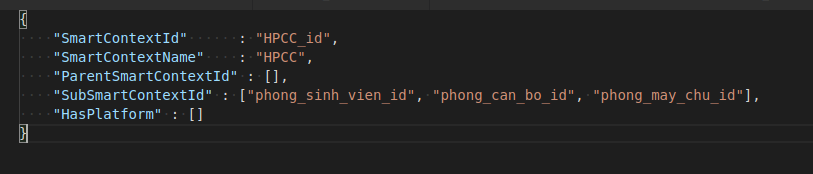
\includegraphics[scale=0.5]{image/smartcontext_instance}
	\caption{Thực thể smartcontext}
\end{figure}

\hspace{0mm}Một thực thể Platform: \\
\begin{figure}[h!]
	\center
	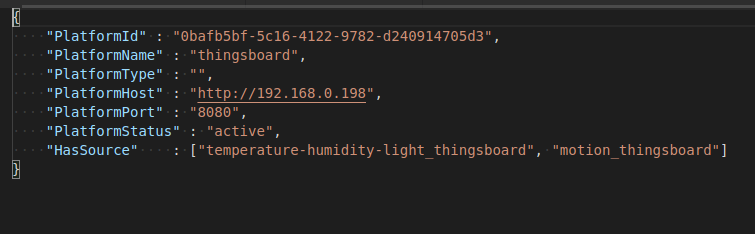
\includegraphics[scale=0.5]{image/platform_instance}
	\caption{Thực thể platform}
\end{figure}

\hspace{0mm}Một thực thể Source:
\begin{figure}[h!]
	\center
	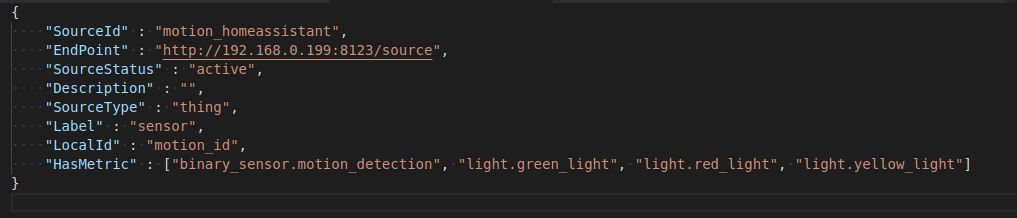
\includegraphics[scale=0.4]{image/source_instance}
	\caption{Thực thể Source}
\end{figure}


\hspace{0mm}Một thực thể Metric:
\clearpage
\begin{figure}[h!]
	\center
	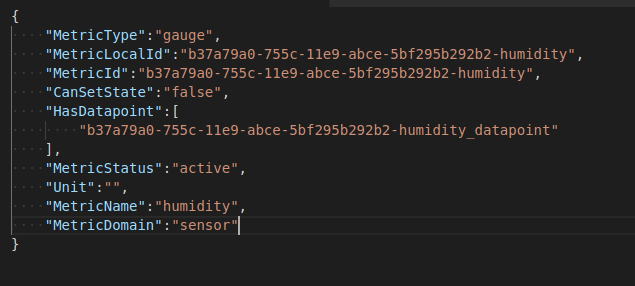
\includegraphics[scale=0.6]{image/metric_instance}
	\caption{Thực thể Metric}
\end{figure}

\hspace{0mm}Một thực thể Data Point:
\begin{figure}[h!]
	\center
	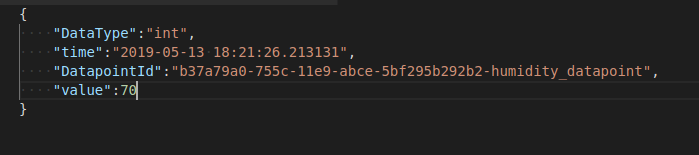
\includegraphics[scale=0.6]{image/datapoint_instance}
	\caption{Thực thể Data Point}
\end{figure}

Sau các bước trên, ta lập được một ontology về lĩnh vực IoT nhà thông minh:
\clearpage
\begin{figure}[h!]
	\center
	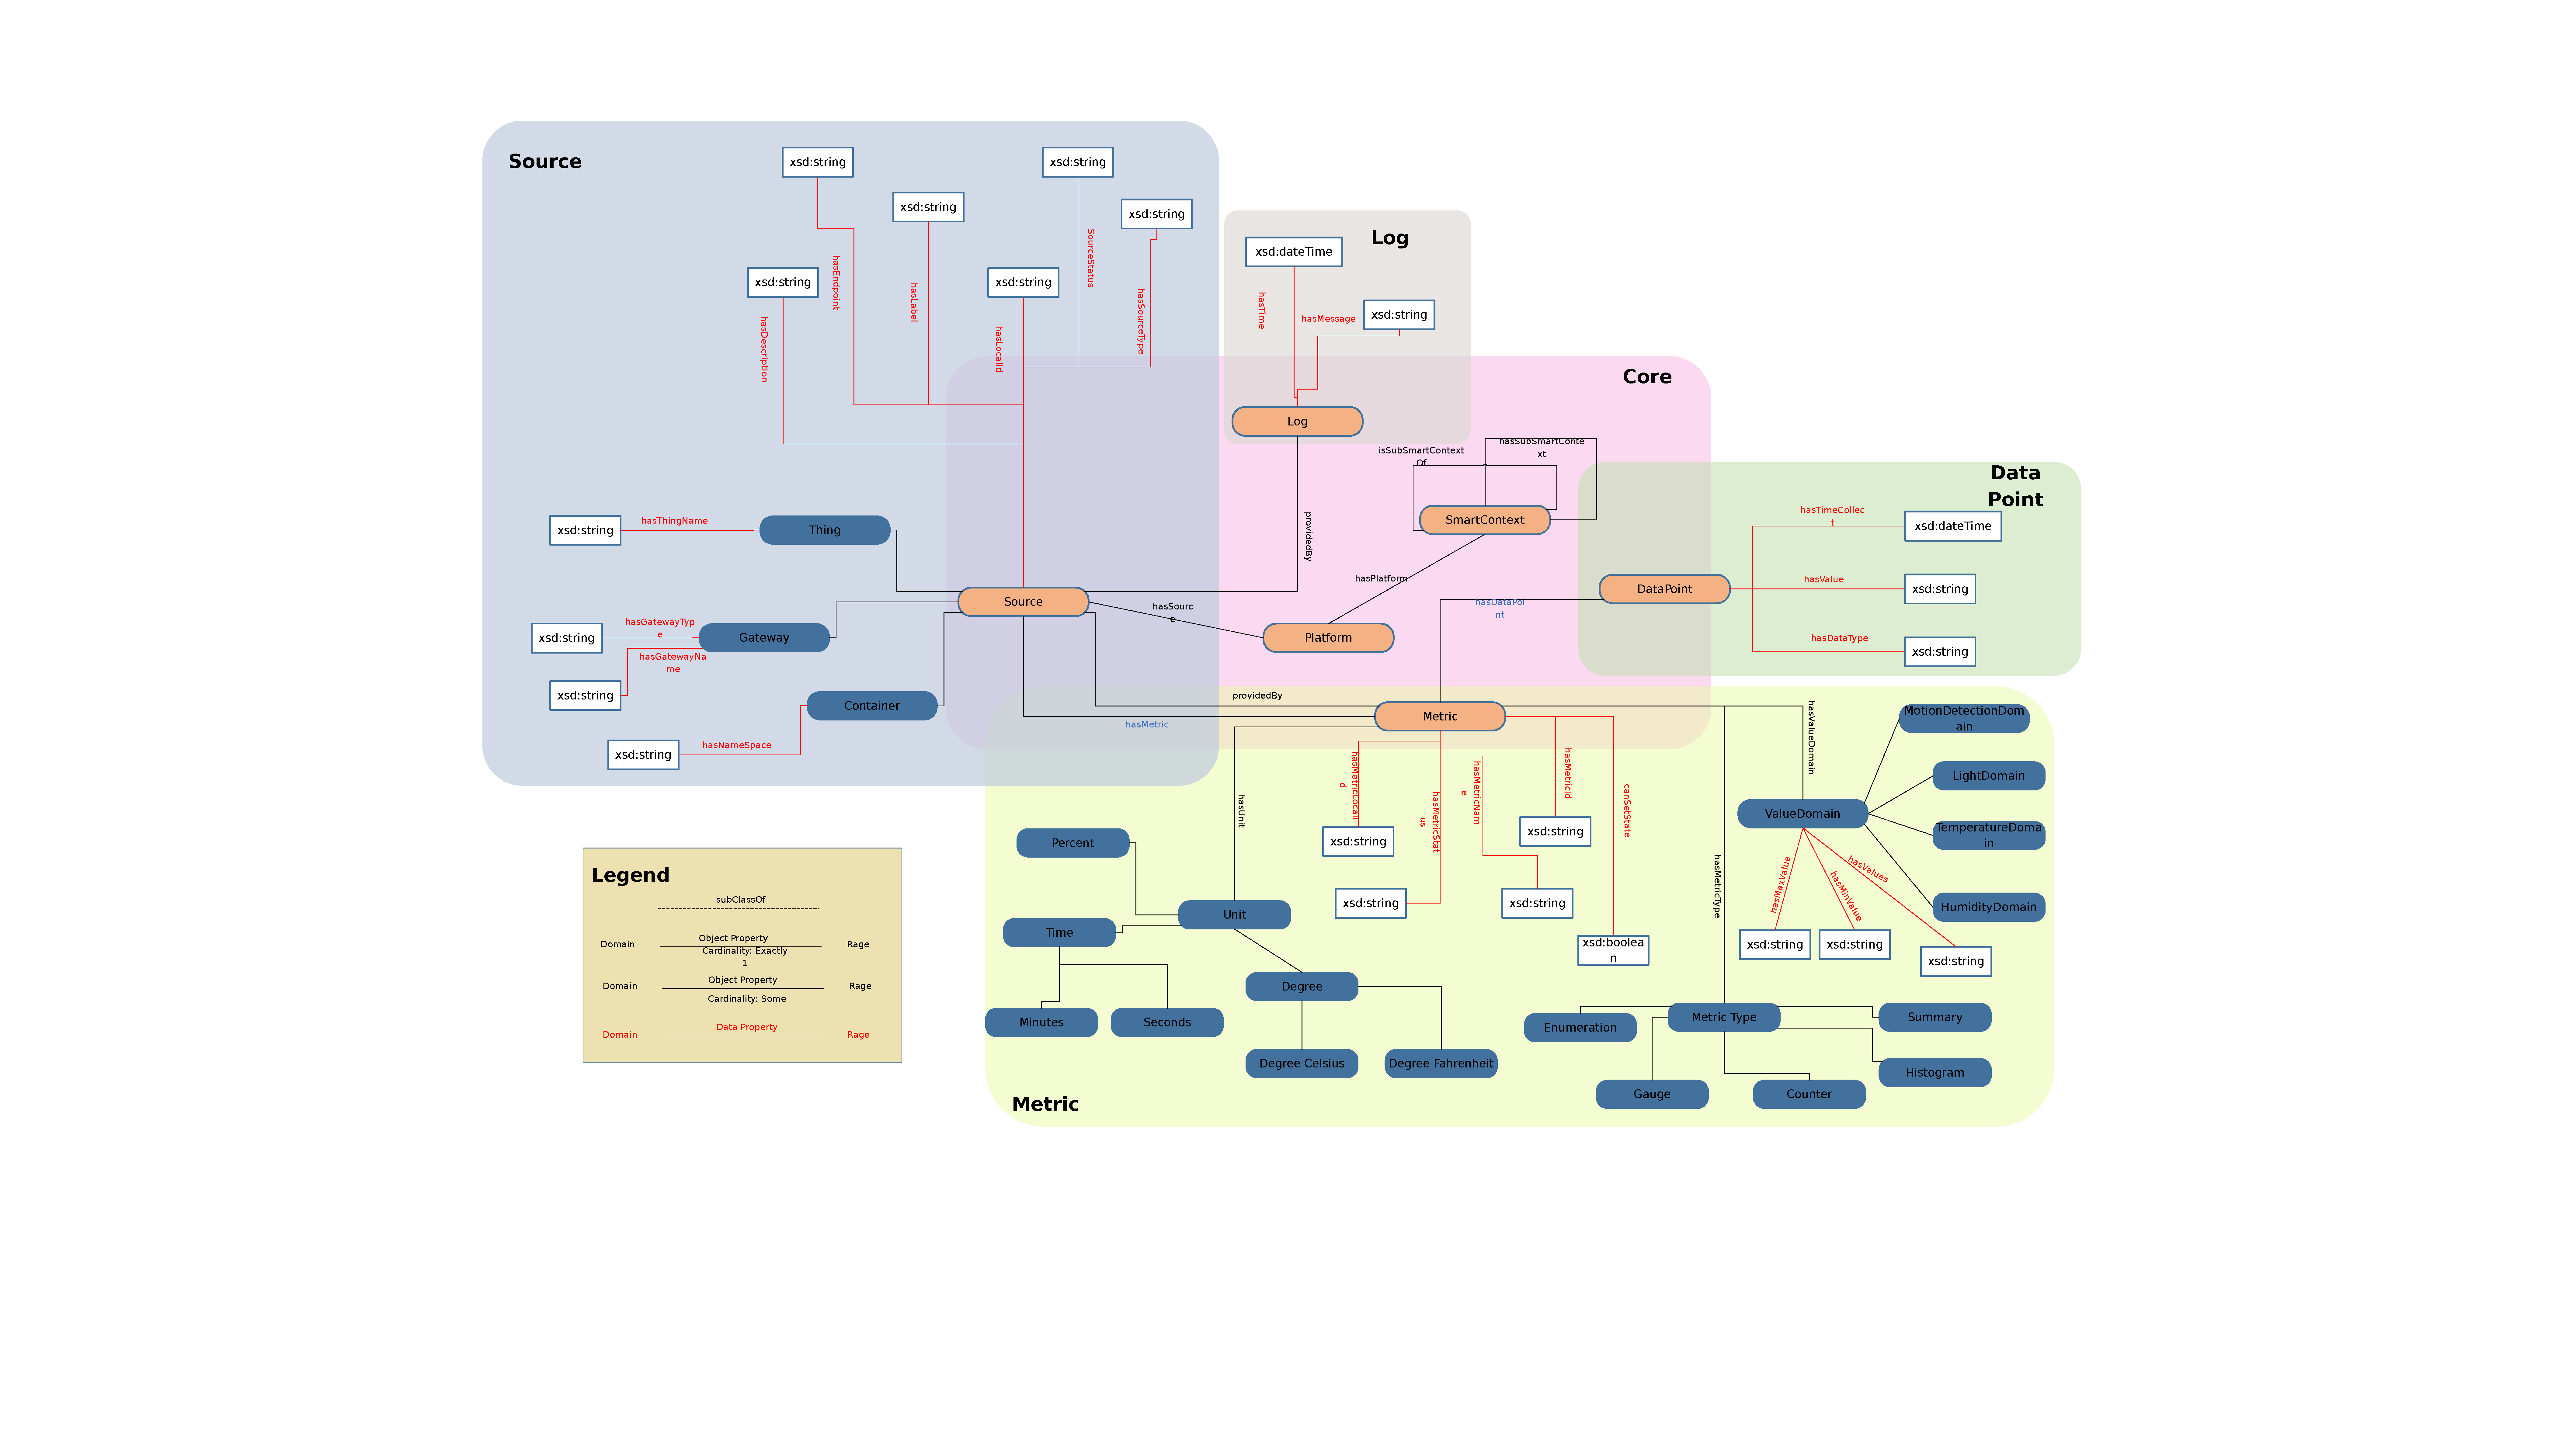
\includegraphics[scale=0.2, center]{image/ontology-2}
	\caption{ontology cho lĩnh vực nhà thông minh}
\end{figure}


\subsection{Cơ chế ánh xạ các dữ liệu trong IoT theo ontology}
Các dữ liệu từ các cảm biến, thiết bị IoT rất khác nhau về cấu trúc. Do trong đề tài này, tất cả các cảm biến, thiết bị đều được gắn với một platform; mỗi platform biểu diễn dữ liệu thu được từ các cảm biến, thiết bị theo một định dạng chuẩn riêng ta phải ánh xạ các định dạng dữ liệu chuẩn của các platform về một dạng chung. Để làm được điều này, ta phải viết các driver cho mỗi platform, nhiệm vụ của driver là ánh xạ định dạng dữ liệu của mỗi platform về định dạng dữ liệu chung của ontology.
Sau khi đã có một định dạng dữ liệu thống nhất, ta phải dùng ngôn ngữ hình thức để biểu diễn các khái niệm trong ontology. Ở đề tài này, tôi dùng định dạng json để biểu diễn các khái niệm, các thuộc tính của các khái niệm cũng như mối quan hệ giữa các khái niệm. 
%\clearpage
\begin{figure}[h!]
	\center
	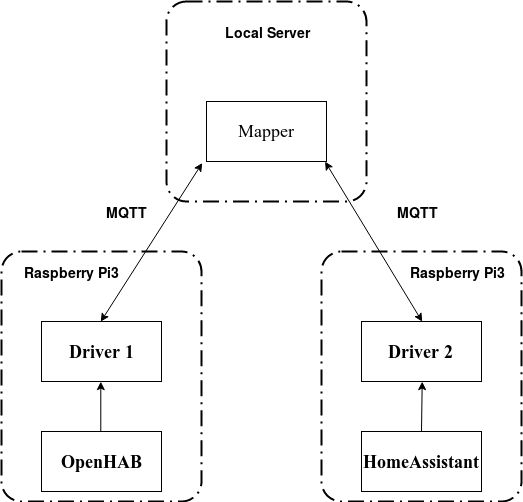
\includegraphics[scale=0.6]{image/mapping_service}
	\caption{Mô hình ánh xạ dữ liệu về một chuẩn của ontology}
\end{figure}

\subsection{Cơ chế truy vấn ngữ nghĩa}
\subsubsection{Biểu đồ use case tổng quát}

\begin{figure}[h!]
	\center
	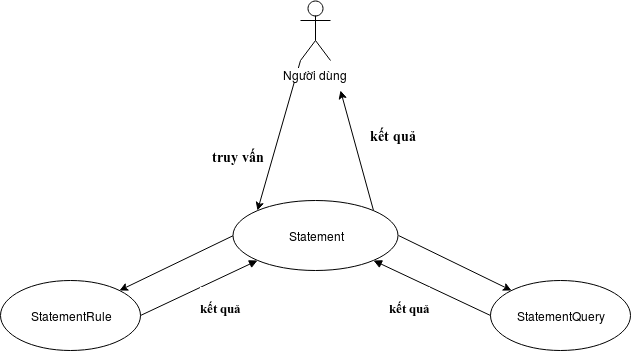
\includegraphics[scale=0.6]{image/language_diagram-use_case}
	\caption{Biểu đồ use case tổng quát}
\end{figure}

\subsubsection{Xây dựng cơ chế truy vấn}
Từ các thực thể được biểu diễn theo ontology, ta phải xây dựng cơ chế để lấy được thông tin của các thực thể, mối quan hệ giữa các thực thể. Để làm được điều này, tôi xây dựng tập các API dựa vào mối quan hệ giữa các khái niệm để đạt được tính ngữ nghĩa. Đồng thời, tôi định nghĩa một ngôn ngữ truy vấn đơn giản, sử dụng tập API trên để tạo ra các câu truy vấn ngữ nghĩa.

Mục đích của ngôn ngữ muốn tạo ra là tạo được các câu truy vấn, tương ứng với nhanh query trong sơ đồ. Để thực hiện câu truy vấn, ta cần chỉ rõ muốn lấy thuộc tính hay khái niệm nào, tập các thuộc tính và khái niệm được gọi là keyword. Ngoài việc chỉ rõ các thuộc tính, khái niệm cần truy vấn, ta cũng cần chỉ rõ điều kiện thực hiện câu truy vấn. Điều kiện này được chứa trong thành phần "Condition". Một chức năng khác mà ta mong muốn ngôn ngữ có thể thực hiện là kiểm tra các điều kiện, nếu điều kiện thỏa mãn thì thực hiện một hành động nào đó, hành động này tương ứng với việc điều khiển các thiết bị IoT dựa trên các API mà các platform cung cấp. Chức năng này được gọi là rule. 
Từ các mục đích trên, ta xây dựng được cấu trúc của ngôn ngữ truy vấn:


\begin{figure}[h!]
	\center
	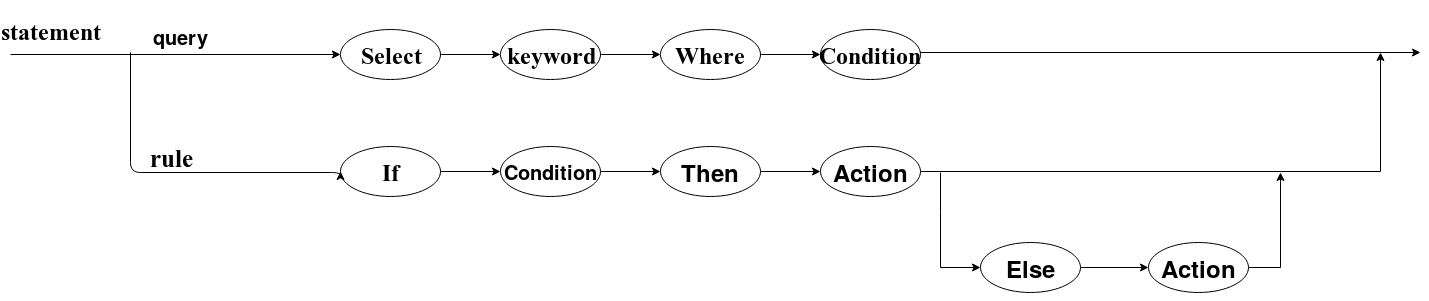
\includegraphics[scale=0.3]{image/language_model-statement}
	\caption{Mô hình ngôn ngữ - statement}
\end{figure}


Một condition là một phép so sánh giữa giá trị tương ứng một keyword với một biểu thức. Ví dụ so sánh PlatformId = "OpenHAB\_id". Các phép so sánh có thể có là <, >, >=, <=, =, !=. Tùy thuộc vào keyword mà có phép so sánh tương ứng. Condition cũng có thể là kết quả của một phép toán logic của một tập hợp các condition khác. Hai phép toán logic hỗ trợ là AND và OR. Ngoài ra, để thể hiện thứ tự ưu tiên của các phép toán logic, ta đưa thêm cặp dấu ngoặc đơn vào ngôn ngữ.

\begin{figure}[h!]
	\center
	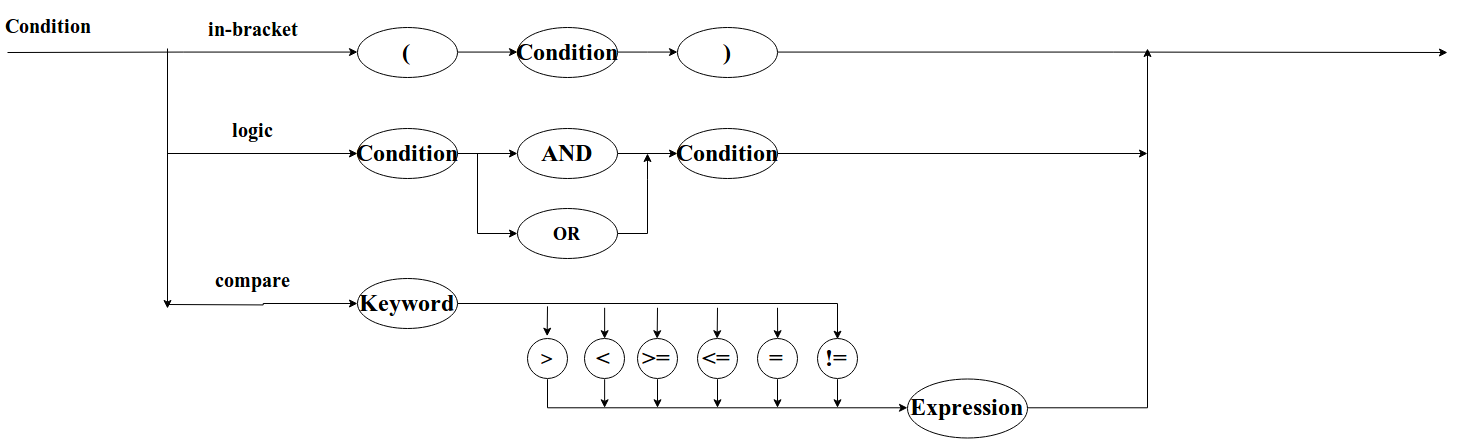
\includegraphics[scale=0.3]{image/language_model-condition}
	\caption{Mô hình ngôn ngữ - condition}
\end{figure}


Một Action (hành động) là một lời gọi tới các API để điều khiển các thiết bị từ nền tảng IoT. Do các thiết bị trong hệ thống chỉ cung cấp hai thao tác điều khiển là bật và tắt nên ngôn ngữ chỉ đưa vào hai hành động là bật và tắt.

\begin{figure}[h!]
	\center
	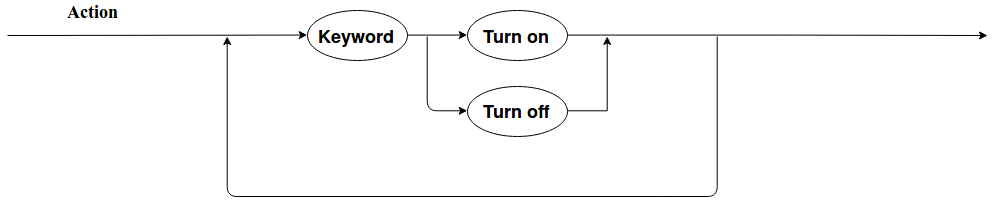
\includegraphics[scale=0.4]{image/language_model-action}
	\caption{Mô hình ngôn ngữ - action}
\end{figure}


Một biểu thức là một toán tử hoặc các phép toán cộng, trừ các toán tử.
\begin{figure}[h!]
	\center
	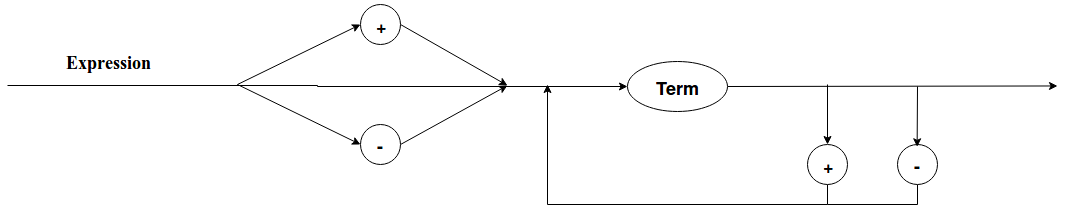
\includegraphics[scale=0.4]{image/language_model-expression}
	\caption{Mô hình ngôn ngữ - expression}
\end{figure}

Một toán tử là một hằng số hoặc các phép toán của các hằng số.
\begin{figure}[h!]
	\center
	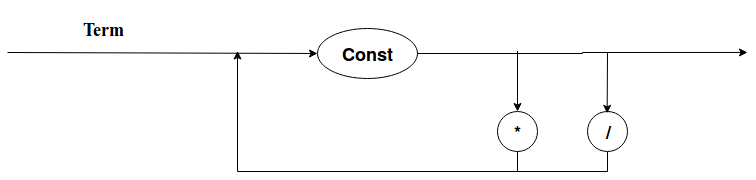
\includegraphics[scale=0.4]{image/language_model-term}
	\caption{Mô hình ngôn ngữ - term}
\end{figure}

Một hằng số là một chuỗi hoặc một số (nguyên hoặc thực).
\begin{figure}[h!]
	\center
	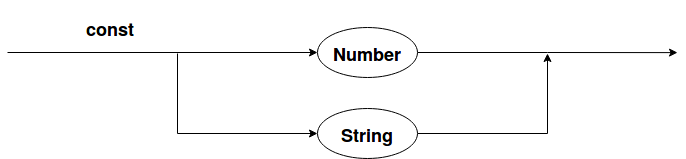
\includegraphics[scale=0.4]{image/language_model-const}	
	\caption{Mô hình ngôn ngữ -const}
\end{figure}
\clearpage

\subsubsection{Biểu đồ lớp của các thành phần của cơ chế truy vấn}

\begin{figure}[h!]
	\center
	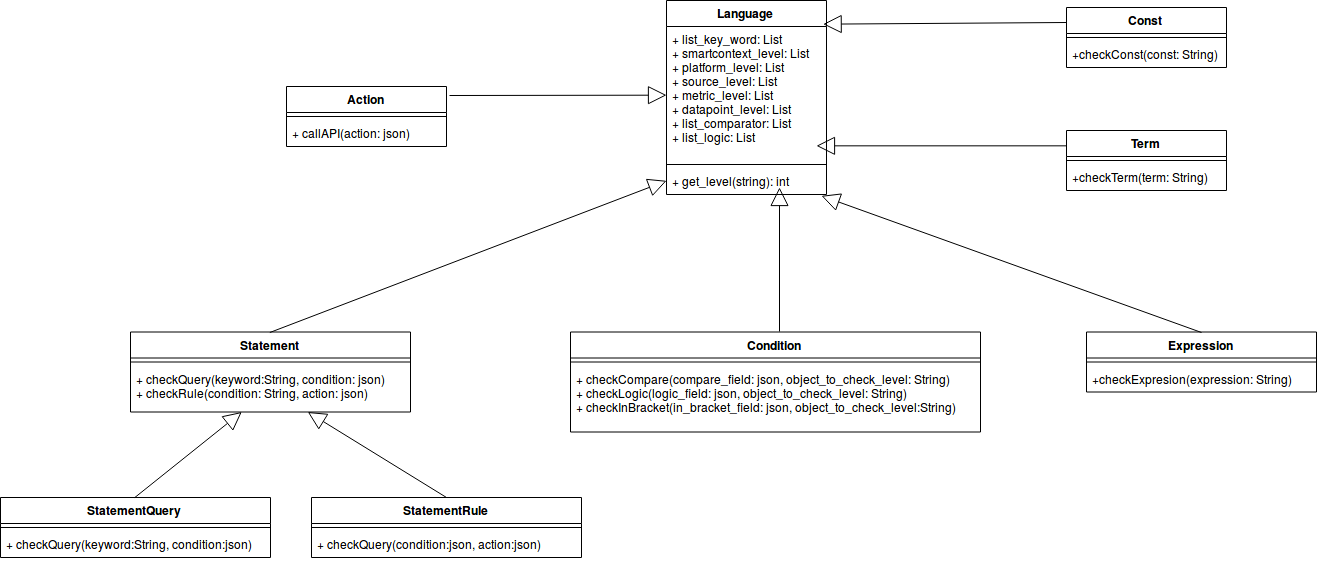
\includegraphics[scale=0.4]{image/language_diagram-class_diagram}	
	\caption{Biểu đồ lớp của các thành phần}
\end{figure}




\subsubsection{Biểu đồ hoạt động các thành phần của cơ chế truy vấn}

\begin{figure}[h!]
	\center
	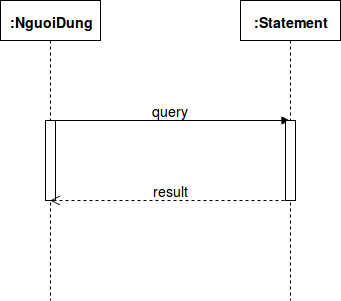
\includegraphics[scale=0.4]{image/language_diagram-statement}	
	\caption{Biểu đồ hoạt động của thành phần Statement}
\end{figure}


\begin{figure}[h!]
	\center
	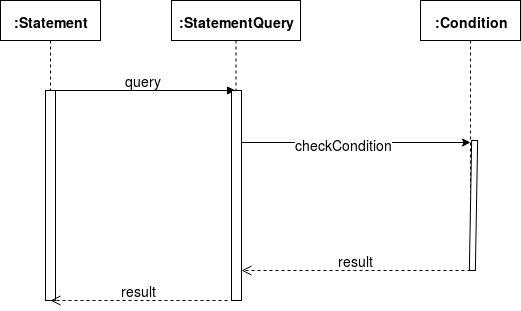
\includegraphics[scale=0.4]{image/language_diagram-statement_query}	
	\caption{Biểu đồ hoạt động của thành phần StatementQuery}
\end{figure}


\begin{figure}[h!]
	\center
	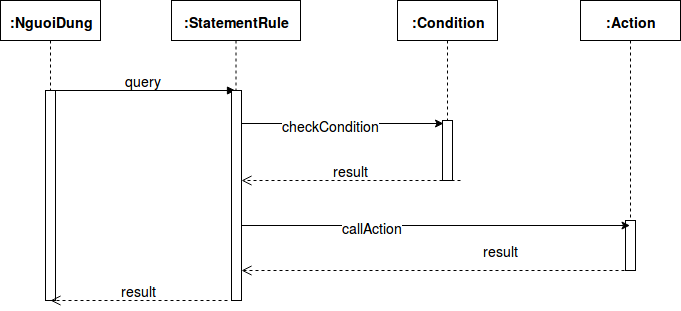
\includegraphics[scale=0.4]{image/language_diagram-statement_rule}	
	\caption{Biểu đồ hoạt động của thành phần StatementRule}
\end{figure}


\begin{figure}[h!]
	\center
	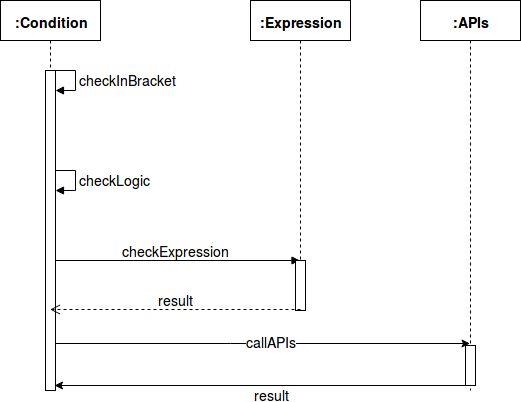
\includegraphics[scale=0.4]{image/language_diagram-condition}	
	\caption{Biểu đồ hoạt động của thành phần Condition}
\end{figure}


\begin{figure}[h!]
	\center
	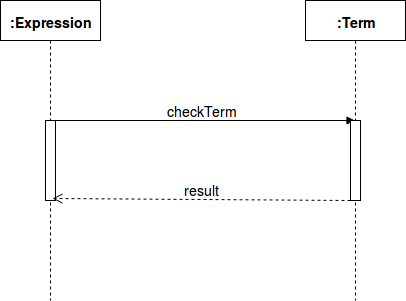
\includegraphics[scale=0.4]{image/language_diagram-expression}	
	\caption{Biểu đồ hoạt động của thành phần Expression}
\end{figure}


\begin{figure}[h!]
	\center
	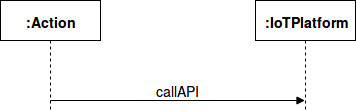
\includegraphics[scale=0.4]{image/language_diagram-action}	
	\caption{Biểu đồ hoạt động của thành phần Action}
\end{figure}


\begin{figure}[h!]
	\center
	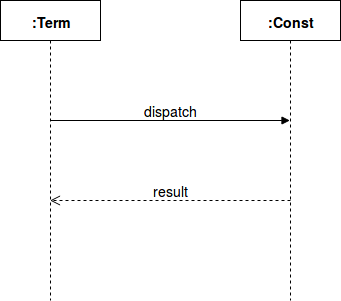
\includegraphics[scale=0.4]{image/language_diagram-term}	
	\caption{Biểu đồ hoạt động của thành phần Term}
\end{figure}


\subsection{Tập các API}
Để cài đặt cơ chế ngữ nghĩa, tôi đã xây dựng tập các API, các API này dựa vào mối quan hệ giữa các khái niệm trong ontology để thực hiện các câu truy vấn ngữ nghĩa. 

Các API cơ bản:

\begin{itemize}
	\item Lấy tất cả các Data Point
	\item Lấy tất cả các Metric
	\item Lấy tất cả các Source
	\item Lấy tất cả các Platform
	\item Lấy tất cả các Smart Context
	\item Lấy tất cả các Smart Context nằm trong Smart Context nào đó. (lấy smart context con)
	\item Lấy tất cả các Smart Context chứa Smart Context nào đó. (lấy smart context cha)
\end{itemize}

Một số API phụ trợ:
\begin{itemize}
	\item Lấy DataPointId/DataPoint của một DataPoint
	\item Lấy MetricId/Metric của một Metric
	\item Lấy SourceId/Source của một Source
	\item Lấy PlatformId/Platform của một Platform
	\item Lấy SmartContextId/SmartContext của một SmartContext
\end{itemize}


Các API thể hiện tính ngữ nghĩa dựa trên mối quan hệ giữa các khái niệm:
\begin{itemize}
	\item Lấy DataPoint từ một Metric
	\item Lấy DataPoint từ một Source
	\item Lấy DataPoint từ một Platform
	\item Lấy DataPoint từ một SmartContext
	\item Lấy Metric từ một DataPoint
	\item Lấy Metric từ một Source
	\item Lấy Metric từ một Platform
	\item Lấy Metric từ một SmartContext
	\item Lấy Source từ một DataPoint
	\item Lấy Source từ một Metric
	\item Lấy Source từ một Platform
	\item Lấy Source từ một SmartContext
	\item Lấy Platform từ một DataPoint
	\item Lấy Platform từ một Metric
	\item Lấy Platform từ một Source
	\item Lấy Platform từ một SmartContext
	\item Lấy SmartContext từ một DataPoint
	\item Lấy SmartContext từ một Metric
	\item Lấy SmartContext từ một Source
	\item Lấy SmartContext từ một Platform
\end{itemize}


Ví dụ về cơ chế ngữ nghĩa trong API: Lấy DataPoint từ một SmartContext.
Để lấy được DataPoint thuộc vào một SmartContext, trước hết ta phải lấy ra các Platform mà Smart Context đó chứa dựa vào mối quan hệ hasPlatform của SmartContext. Khi đã xác định được các Platform, với mỗi Platform, xác định xem nó chứa các Source nào dựa vào mối quan hệ hasSource của Platform.Với mỗi Source, xác định xem nó chứa các Metric nào dựa vào mối quan hệ hasMetric của Source. Với mỗi Metric, xác định DataPoint mà nó chứa dựa vào thuộc tính hasDataPoint của Metric. Vậy sau khi duyệt qua các quan hệ trên ontology, ta sẽ lấy ra được các DataPoint nằm trong một SmartContext. Cơ chế truy vấn ngữ nghĩa này hoàn toàn tương tự đối với các API khác được xây dựng.